\documentclass[a4paper,12pt]{article}
\usepackage{fullpage}
\usepackage[british]{babel}

\usepackage{amsmath}
\usepackage{amssymb}
\usepackage{amsthm} \newtheorem{theorem}{Theorem}
\usepackage{color}
\usepackage{float}
\usepackage{listings}
\usepackage{subfig}
\lstset{% parameters for all code listings
	language=Python,
	frame=single,
	basicstyle=\small,  % nothing smaller than \footnotesize, please
	tabsize=2,
	numbers=left,
	framexleftmargin=2em,  % extend frame to include line numbers
	%xrightmargin=2em,  % extra space to fit 79 characters
	breaklines=true,
	breakatwhitespace=true,
	prebreak={/},
	captionpos=b,
	columns=fullflexible,
	escapeinside={\#*}{\^^M}
}
\usepackage{fancyvrb}
\DefineVerbatimEnvironment{code}{Verbatim}{fontsize=\small}
\DefineVerbatimEnvironment{example}{Verbatim}{fontsize=\small}

\usepackage{tikz} \usetikzlibrary{trees}
\usepackage{hyperref}  % should always be the last package

% useful colours (use sparingly!):
\newcommand{\blue}[1]{{\color{blue}#1}}
\newcommand{\green}[1]{{\color{green}#1}}
\newcommand{\red}[1]{{\color{red}#1}}

% useful wrappers for algorithmic/Python notation:
\newcommand{\length}[1]{\text{len}(#1)}
\newcommand{\twodots}{\mathinner{\ldotp\ldotp}}  % taken from clrscode3e.sty
\newcommand{\Oh}[1]{\mathcal{O}\left(#1\right)}

% useful (wrappers for) math symbols:
\newcommand{\Cardinality}[1]{\left\lvert#1\right\rvert}
%\newcommand{\Cardinality}[1]{\##1}
\newcommand{\Ceiling}[1]{\left\lceil#1\right\rceil}
\newcommand{\Floor}[1]{\left\lfloor#1\right\rfloor}
\newcommand{\Iff}{\Leftrightarrow}
\newcommand{\Implies}{\Rightarrow}
\newcommand{\Intersect}{\cap}
\newcommand{\Sequence}[1]{\left[#1\right]}
\newcommand{\Set}[1]{\left\{#1\right\}}
\newcommand{\SetComp}[2]{\Set{#1\SuchThat#2}}
\newcommand{\SuchThat}{\mid}
\newcommand{\Tuple}[1]{\langle#1\rangle}
\newcommand{\Union}{\cup}
\usetikzlibrary{positioning,shapes,shadows,arrows}


\title{\textbf{Evolutionary Simulator In A Dynamic Environment}}

\author{Jonathan Sharyari \and Lukas Klingsbo}  % replace by your name(s)

%\date{Month Day, Year}
\date{\today}

\begin{document}

\maketitle

\section{Abstract}
Genetic algorithms (GAs) are a well established optimization tool for static problems. Recently, genetic algorithms have been proposed to improve the adaptivity of GAs in dynamic environments. In this paper, we attempted to implement and compare some of these methods; two methods based on mutation, and two based on periodic insertions of \emph{immigrants}. Although there was not enough time to perform extensive comparisons of the algorithms, a test environment was developed that is extensive and easily available.


\section{Introduction}
Genetic algorithms are a common tool to find solutions to complex problems, often with high dimensionality. Although much research has been done on the subject, this research has to some extent focused on problems in a stationary environment.

Since in a dynamic environment, the fitness function changes over time a traditional GA is not very suited for solving dynamic problems, as it is likely that the population will quickly converge and not be able to adapt when the fitness function changes.

Several approaches have been proposed in order to allow GAs to maintain the population diversity, two common methods are \emph{random} or \emph{elite immigrants} and \emph{triggered hypermutation} [1][2].

The goal of this project is to evaluate the methods proposed in earlier work, on a dynamic environment designed for the purpose.

\section{Environment}
Our test environment consists of a simple map containing clusters of "food", and is initialized randomly. The goal of the population is to find paths leading to areas where the food is distributed. A dynamic environment is created by changing the positions of the food in the map. This can be done in many ways, and we settle for three different methods of changing the map.

\begin{itemize}

\item
Slightly changing - Small changes are done, but fairly often. The optimum after a change will lie close to the earlier optimum.
\item
Abruptly changing - The map is reinitialized, changing the positions of obstacles and enemies. This must be done rarely, as to give the population the time to re-adapt.
\item
Seasonally changing - similar to abrupt changes, the changes are large and rare, but the number of maps is finite and periodic.
\end{itemize}

We anticipate that the different dynamic methods tested (explained below) will perform differently depending on the type of dynamic maps used.

\section{Suggested Dynamic Methods}
\subsection{Hypermutation}
The concept of mutation is critical for genetic algorithms, as it is through mutation a genetic algorithm maintains its diversity. As the problem of training in a dynamic environment is to avoid or overcome early convergence, it is tempting to try training with a higher degree of mutation than commonly used in static environments. Although this is a simple concept, [1] shows that this method can generate relatively good results.

\subsection{Triggered Hypermutation}
A higher mutation rate results in higher diversity as indicated above, but a high mutation rate makes it more difficult to converge. The mutation rate is therefore generally kept low in standard GAs. The method of using a high mutation rate in a dynamic system might therefore lead to non-converging individuals.

Triggered hypermutation is a proposed solution to this problem. The mutation rate in general is kept low, giving better convergence. When the system is altered in a way that decreases the fitness, the hypermutation stage is started and the mutation rate is temporarily increased giving the same effect as the method explained above.

The results in [1] and [2] show that this method is efficient when the changes in the environment are small, but does not cope as well with abrupt changes.
\subsection{Immigrants}
Random immigrants and elitism-based immigrants use a different approach to maintain diversity. In these methods, some individuals with low fitness are removed and replaced with new individuals.

With random immigrants, these new individuals are randomly created (by the same method individuals were initialized at the beginning).

With elitism-based immigrants, the individuals with high fitness are remembered. When the total fitness decreases (potentially due to changes in the environment), individuals with low fitness are removed and individuals from this elite-set are reintroduced.

The random immigrants method has been shown to be beneficial for most dynamic environments, compared to the standard GA, but not necessarily the best method[3]. Using elite immigrants, the results can be improved for slightly changing and seasonal environments, but as this method keeps a lower diversity, it does not perform as well when the changes are more abrupt.

\section{Genome representation}
The behavior of an individual depends on its genome, which decides how it moves on the map. The genome is represented as a matrix of vector values where each position in the matrix represents a part of the map, and the vector stored at the position is the direction in which the individual will move. For a matrix of size $m \times n$, this is represented as m arrays of size n.

Consider a map of size $50m \times 50n$ and a matrix of size $m \times n$. Then every matrix position will represent a $50\times50$ square in the map. When the individual has a position inside that square, it's speed and direction will be given by the vector stored in that position of the matrix.

\section{Selection and Crossover strategies}
Two different crossover types were used, epoch and collision learning. In collision learning, the individuals crossover when they collide in the map, provided they have collected some fixed amount of food. Two new individuals are created by one either one-point, two-point or uniform crossover.

This type of crossover was useful during implementation, as the results could easily be seen graphically. But as this is not a traditional way of selection, epoch learning was used as only then could the implementation of the above methods be done in a way that is comparable with the result in previous research.

In epoch learning, the individuals search the map for a fixed set of updates, one epoch. At the end of the epoch, individuals were re-combinated and mutated depending on the settings used. The selection method used worked by first sorting the list of individuals, with the highest fitness first, using the number of food collected as a measure of the fitness. Then, each individual from the beginning crosses over with a probability $\alpha$ with the first individual. If not, the individual crosses over with the same probability $\alpha$ with the second individual, and so on. In general, only the best half of the individuals reproduce.

\section{Results}
As this project had a short time limit, we were not able to perform rigorous testing of the methods. One thing that could be seen was that random immigrants improved convergence in dynamic maps with abrupt changes, a result that is in line with the results in [3]. 

In order to perform testing, a graphical web-interface was created. This interface can for a limited time be reached at http://mindlevel.net. This interface also gives an indication of the standrad settings used during testing.

\section{Discussion}
\subsection{genome representation}
The genome is represented as an array of arrays. During a crossover, assume 1-point, the crossover will be row by row until the point of crossover, but could not be column by column. This means the convergence with this representation will be much more effective if the target (the food) lies in a horizontal line from their starting position, than if they lie in a vertical line. See illustration.

\begin{figure}[h!]
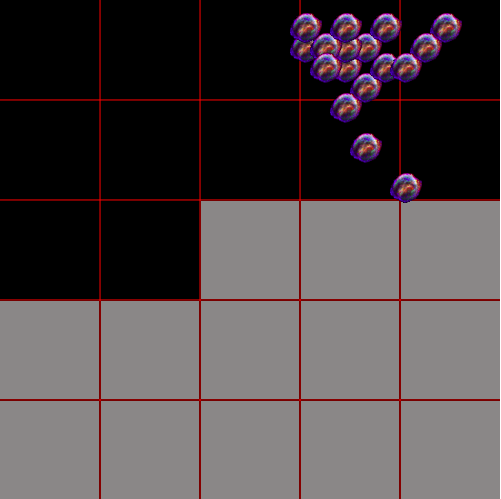
\includegraphics[width=0.4\textwidth]{TopRight.png}
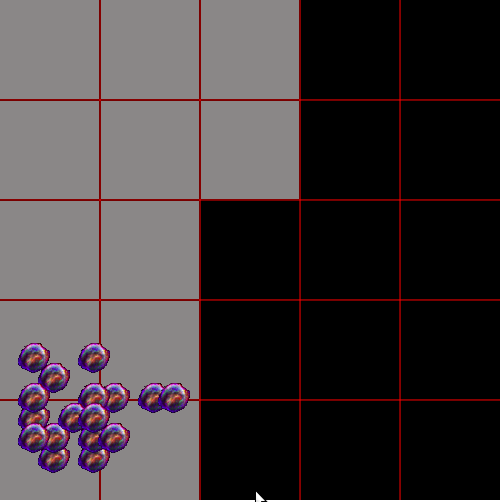
\includegraphics[width=0.4\textwidth]{BottomLeft.png}
\caption{The map in the left pictures is "easier" than the map in the right picture, even though one map is a rotation of the other. This is because the 1-point crossover illustrated to the left is possible with our representation of a genome, but the crossover to the right is not.}
\end{figure}

By randomly changing the starting position of the individuals at the start of each epoch, the impact of this bias is lowered, as it is as as likely that the individuals will spawn with the food along a horizontal line from their position, as along a vertical line.

\section{Proposed Future Work}
During the time of work, there was not enough time to perform comparisons of the different methods. A proposed method on how this could be done is to find for each method (standard GA, triggered hypermutation, elitism-based immigrants and random-immigrants) and for each type of environment (static, evolving, shotgun and seasonal) find a set of parameters that seem to give the best result.

Then, each method and environment type combination could be tested on the same maps a large number of times, to minimize the variance of the performance. Using this, a good measure of the performance could be obtained from which better conclusions could be drawn.

%It is likely that the immigrant-based methods and the standard GA would have similar optimal parameter settings, due to the fact that the algorithms change little of the standard GA. 



\section{references}
[1] H. G. Cobb, J. J. Grefenstette (1993)

Genetic Algorithms for Tracking Changing Environments

Proceedings of the 5th International Conference on Genetic Algorithms

[2] A. Simões, E. Costa (2002)

Using Genetic Algorithms to Deal with Dynamic Environments: A Comparative Study of Several Approaches Based on Promoting Diversity

GECCO '02 Proceedings of the Genetic and Evolutionary Computation Conference

[3] S. Yang (2007)

Genetic Algorithms with Elitism-Based Immigrants for Changing Optimization Problems

Lecture Notes In Computer Science, 2007, volume 4448, pages 627-636
\end{document}

